%-------------------------------------------------------------------------------
% File: usage.tex
%
% Author: Marco Pinna
%         Created on 14/07/2022
%-------------------------------------------------------------------------------
\chapter{Usage}\label{ch:usage}
This chapter shows some examples of usages, both for the voter and for the administrators of the system.\\

\section*{Voting}
Upon entering the polling booth, the voter is presented with the screen shown in \ref{fig:login}.\\

\begin{figure}[H]
    \begin{center}
        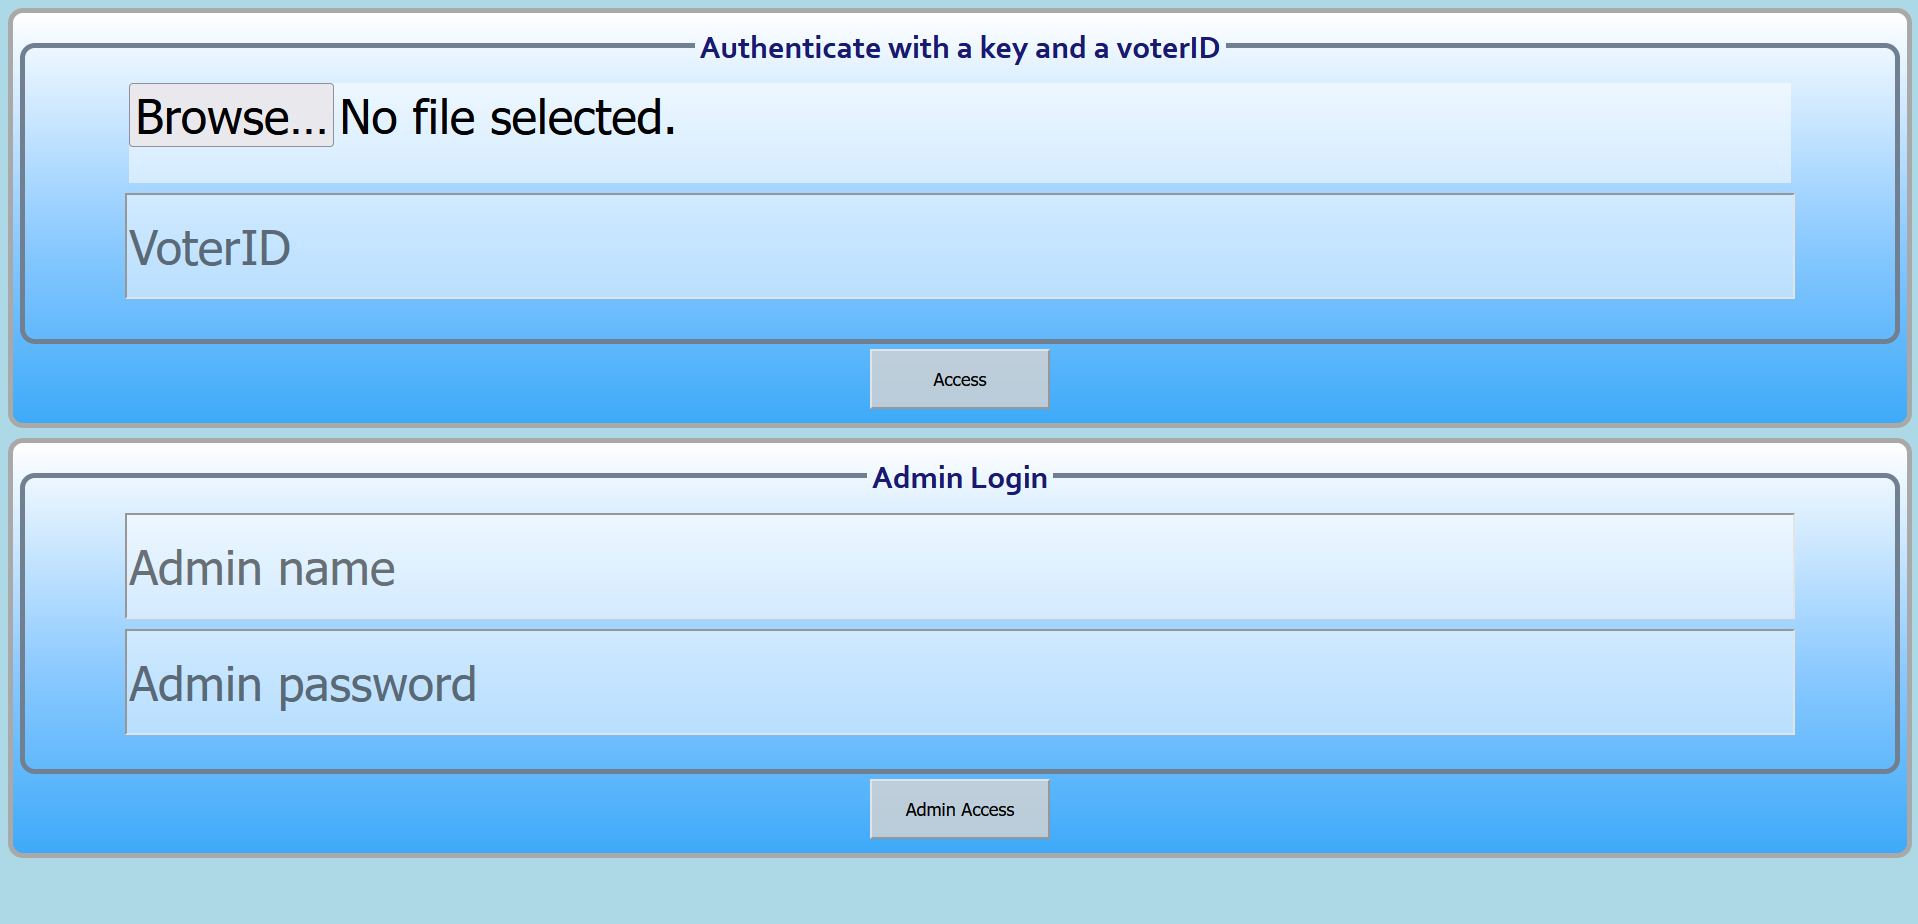
\includegraphics[scale=0.4]{img/login.png}
    \end{center}
    \vspace*{-0.5cm}
    \caption{Screenshot of the login page of the polling booth device.}
    \label{fig:login}
\end{figure}

For the sake of demonstration, the voter here is required to upload a file containing their private key, but in the actual procedure this step would be carried out with an electronic document, dedicated hardware and no need to upload any file.\\
After logging in, the voter is redirected to a new page containing the digital ballot paper. It contains a form with all the possible candidates that can be chosen but also a field in which they can write freely to guarantee the possibility of sending a blank ballot.\\

\begin{figure}[H]
    \begin{center}
        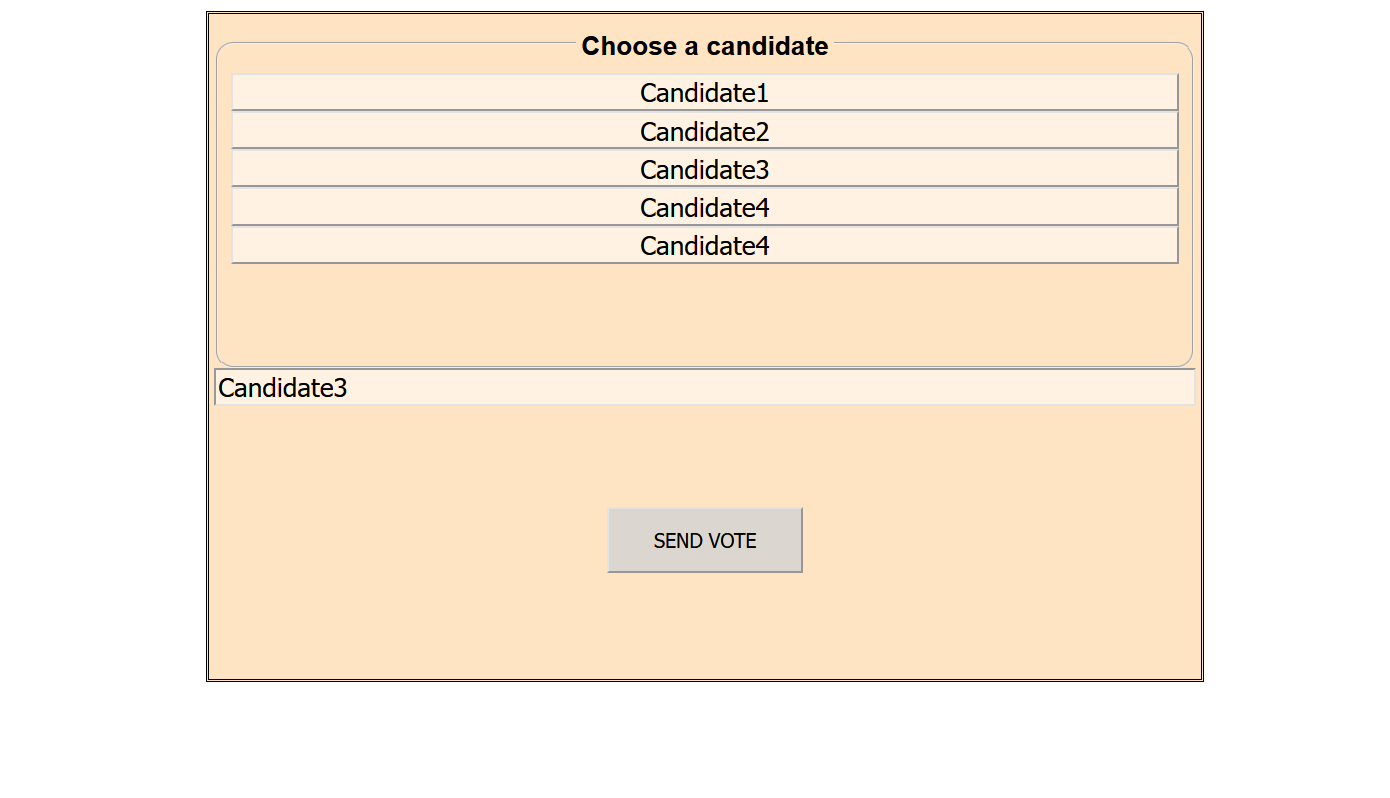
\includegraphics[scale=0.6, trim={3cm 0 3cm 0},clip]{img/ballot.png}
    \end{center}
    \vspace*{-0.5cm}
    \caption{Screenshot of the ballot page.}
    \label{fig:ballot}
\end{figure}
\pagebreak
\section*{Management}
The polling station administrator can access a management dashboard by providing admin credentials to the login page.\\
The dashboard appears as shown in \ref{fig:dashboard}

\begin{figure}[H]
    \begin{center}
        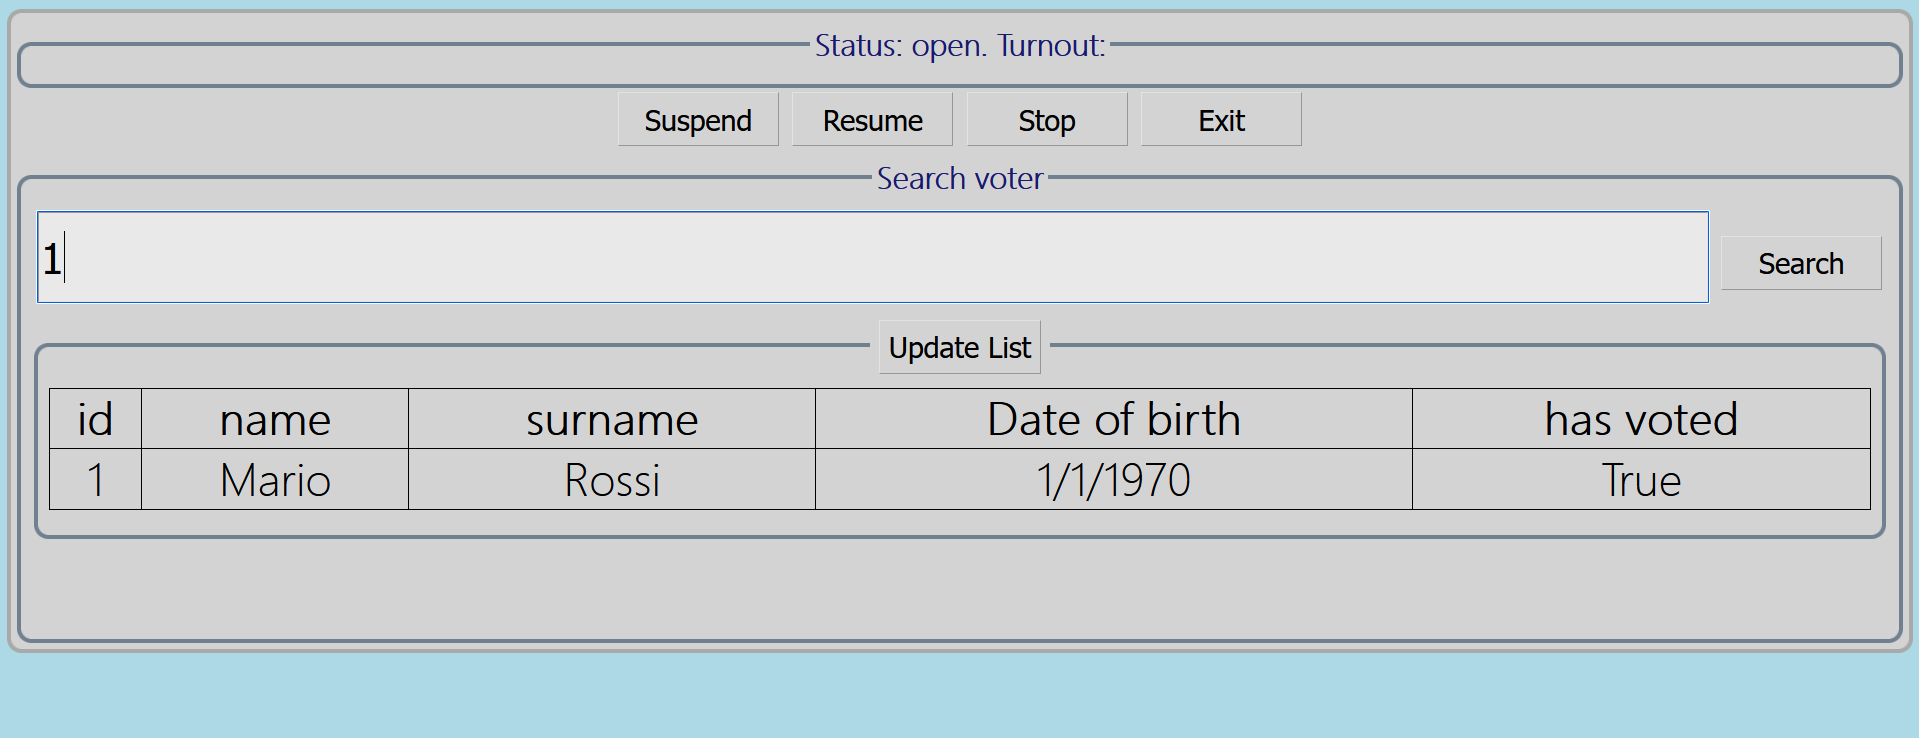
\includegraphics[scale=0.4]{img/dashboard.png}
    \end{center}
    \vspace*{-0.5cm}
    \caption{Screenshot of the admin dashboard.}
    \label{fig:dashboard}
\end{figure}